\section{Setting up port I/O}



The AVR ATMEGA88P (and many other series of the AVR chip) include integrated pull-up resistors coupled to the I/O pins for use in active-low inputs. This is very useful as it allows us to make use of these pins without adding complication to the circuit with external resistors, and without having to be concerned over whether or not the state of these pins is known.

The PORTC register contains the A/D converters on most pins, this register will be used for A/D only. The specific input will vary with the function of the entire device itself (DC voltage, DC current work on separate pins, etc.)

We determine the A/D converter to activate by reading the inputs on PORTB. Only 4 of the PORTB pins are used (PB0, PB1, PB2, PB3) as only 4 bits of information are needed. Initializing these pins is done by specifing the data direction register to input on those 4 pins, and writing logic ones to them. Writing a logic one to an input pin causes the AVR to activate the internal pull-up resistor to that pin.

\begin{lstlisting}		%This is for inserting code bits straight into Latex
DDRB = 0b11110000;
PORTB = 0b00001111;
\end{lstlisting}

Determining the "switch" position was done by reading the values of PORTB and then masking off the certain bits we don't care about for that purpose (as far as I know, this is the only way of doing this, as the AVR will not allow individual pin access without reading the entire port.) An example of one of the switch conditions used is shown below, all of them are in a similar format to this one.

\begin{lstlisting}
while(PORTB&_BV(0) == 0){
\end{lstlisting}

One of the sources of significant problems as the use of serial communication to the PC to check the output on the LCD (the idea being to be able to compare output that comes back to minicom to what comes out on the LCD.) However, the LCD never worked correctly under these test conditions. PORTD is used as our data register for writing to the LCD, but it is also used in the serial USART communications, and setting up the serial and running it in parallel with the LCD output consistently produced garbage output.

After the serial communication was removed (ironically from the program designed to test the LCD output) the LCD did properly output characters, perform shifts, etc. Be extremely careful about multi-purposing ports on the chip, and be sure to know you're doing it!
\clearpage
\section{Analog scaling hardware}

The analog component of this device consists of two differential operational amplifiers. One is used for the voltage measurements and calculations, and the other is used for current sensing over the sense resistor. The sense resistor is 5 5$\Omega$ resistors in parallel (forming a 1$\Omega$ resistor). The current sensing amplifier has a differential gain of one, and is setup for minimal common mode gain.

\begin{equation}
\label{3:eq:Acm}
	R1 = R3+R4
\end{equation}

This is to minimize common mode gain by matching the input impedance at each terminal of the amplifier. In order to make sure the differential gain is set appropriately, the feedback resistors need to be scaled to the input resistors.

\begin{equation}
\label{3:eq:Ad}
	\frac{R2}{R1} = \frac{R4}{R3}
\end{equation}

\begin{figure}[h]
	\centering
	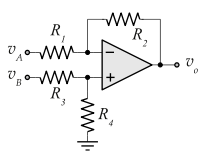
\includegraphics[width=0.40\textwidth]{genericdiffamp}	
	\caption{Generic differential amplifier}
	\label{3:fig:gdamp}
\end{figure}

Our specific differential amplifier schematics are included in the attachments. The current amplifier would probably be better served by an instrumentation amplifier (as a gain of 1 is required), but this was unavailable at the time.

The voltage amplifier functions more like an attenuator for this circuit, the amplifier is setup for a differential gain of 1/200, to allow for measuring of voltages far in excess of 1.1V (the aim of this being able to measure at least 170-200V). As a differential amplifier, this should not expose dangerously high voltages to the operational amplifier (as the majority of the voltage will be dropped over the input resistor, leaving a safe level (<5V) to be dropped over the feedback resistor $R_2$ or ground resistor $R_4$. An instrumentation amplifier could not be used for this, as it is impossible to achieve a gain of less than from that type of device.

Differential amplifiers naturally invert the output, so the positive lead would go into the negative terminal of the amplifier, and vice-versa. This solution (probably foolishly) in its current state relies on the user to correctly apply the input probes so that the output from the amplifier is positive, IE: he knows which voltage is expected to be higher. The voltages coming out of the amplifier however are relatively low (<1.1V), so they should not damage the ADC. Obviously, being able to read negative voltages sometimes would be necessary to do AC analysis, but we could not determine the ADC output to determine the reference, as we never got output from them (even before testing with these waves or any kind of negative signal to the ADC